%!TEX root = ../thesis.tex
%*******************************************************************************
%****************************** Second Chapter *********************************
%*******************************************************************************

\chapter{Deep Learning}

\ifpdf
     \graphicspath{{Figs/Chapter2/}}
\else
    \graphicspath{{Chapter2/Figs/Vector/}{Chapter2/Figs/}}
\fi

There are many tasks which are hard to write algorithms for. For example, writing an algorithm the identifies a type of fruit using a picture of the fruit is a challenging undertaking. You could try to solve this problem by asking a number of yes or no questions which help whittle down the possibilities to a handful of fruit. A sensible question to ask might be - "Is the fruit round?". If the answer was yes, we could immediately discard options like strawberries, pineapples and pears. Another sensible question to ask might be - "Is the fruit orange?". If the answer is yes, again we could immediately discard unlikely candidates. Finally we could ask - "Is the fruit rough?". And if the answer was no, we could be pretty sure the picture we were looking at was an orange. \newline
The problem with this approach is that it is very brittle. You could ask a question that would lead a high likelihood that the image was indeed an orange, however the image may not in fact be an orange. For example apples could also be round, orange and smooth. More questions could try to disambiguate the two types of fruit, but there is enough variation in fruit that our algorithm could be confused. Writing rules in this way also is not scalable. There are a large number of types of fruits, and writing questions to determine each one quickly becomes intractable, let alone questions that help distinguish similar fruit. \newline 
Machine learning (ML) is used to solve such tasks, as well as others such as weather prediction, stock price forecasting and risk modelling ~\citep{hastie2009elements}. ML is the process of using data to build prediction models where these models typically output discrete (classification) or continuous (regression) values. ML uses a number of learning paradigms ~\citep{murphy2012machine}, including supervised learning, unsupervised learning and reinforcement learning, to train models. The models can be divided into three classes, namely shallow, deep and probabilistic ~\citep{hastie2009elements, murphy2012machine}. The models are trained using data to accomplish a task. \newline
\newpage
This chapter presents a discussion on the supervised learning paradigm, an analysis of the convolutional network ~\citep{lecun1998gradient} and recurrent network ~\citep{werbos1988generalization} deep learning models, and a discussion on deep learning training techniques, including dropout ~\citep{srivastava2014dropout} and batch normalisation ~\citep{ioffe2015batch} regularisation. 


%********************************** %First Section  **************************************

\section{Supervised Learning}

ML prediction models take as input a set of features. These features are attributes of a data sample. For example in the fruit prediction task mentioned above, input features would be the attributes of a fruit. They would include characteristics such as shape, colour, texture and size. These inputs are provided to a model that maps to outputs. In the example above, these outputs would be types of fruit, and could represent values such as oranges, apples, strawberries and pineapples, amongst others. The model is then taught (trained) to identify the correct fruit (output) based on the features (input) it receives. This type of training paradigm is called supervised learning \citep{bishop2006pattern, hastie2009elements, murphy2012machine}. \newline

\begin{figure}[H]
  	\caption{Supervised Learning}
   	\centering
    	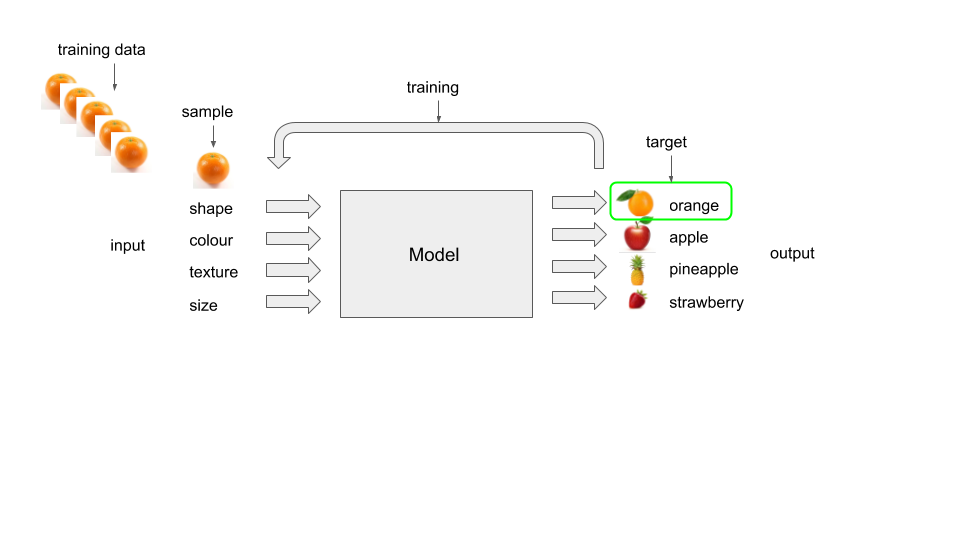
\includegraphics[width=\textwidth]{supervised_learning}
\end{figure}

Features can be continuous valued or discrete, where discrete values are referred to as categorical variables. Outputs can also be continuous or discrete, where discrete outputs are known as labels. Input-output pairs comprise a dataset which is represented as follows, \begin{math} D = \{(x_i, y_i)\}_{i=1}^N \end{math}, where \begin{math} D \end{math} is the dataset, \begin{math} x_i \end{math} is the input sample and \begin{math} y_i \end{math} is the output. The model has to learn the correct mapping of input to output - features to label. We use data samples to train the model to recognise which features are correlated with which labels. The model is trained using an algorithm where it is shown a sample and it outputs what it believes is the correct label. If it gets the label wrong, an objective function is used to assess how large the error was, and the model is adjusted. The algorithm is expressed as follows: \bigbreak

\begin{algorithm}[H]
	\SetAlgoLined
	\textbf{Input} 
	Training set \begin{math} D = \{(x_i, y_i)\}_{i=1}^N \end{math}, samples and labels\;
  	\begin{math} S_{batch} \gets sample(S, b) \end{math} // sample a minibatch of size \begin{math} b \end{math} \\
	 \For{(x, y) \begin{math} \in S_{batch} \end{math}}{
     		\begin{math} y \gets predict(x, y) \end{math} // predict label for sample \\
		\begin{math} e \gets y' - y \end{math} // compute error
     		}
	Update model w.r.t. \begin{math}  e \end{math}
	\caption{Supervised Learning}
\end{algorithm} \bigbreak

%Loss surface image
We try to minimise this error during training, and because we try to minimise the objective function value, it is called a loss function. \newline

The computed class, represented as a logit magnitude, is compared against the target class and an objective is defined that is to be minimised. The logit magnitude is then typically passed through a thresholding function, a softmax function \cite{reference} if a proper probability is desired, or a sigmoid \cite{reference} if only a likelihood is required. Two techniques are used to simultaneously improve both variance and bias respectively: batch normalisation \cite{reference} and dropout \cite{reference}. \newline 

%Classification decision boundary example


%********************************** %Second Section  **************************************

\section{Deep Learning Modes}

\subsection{Convolutional Networks}
The state-of-the-art in deep learning classification models is convolutional neural networks (CNN) \cite{reference}. CNNs are typically applied to object classification within images, and take advantage of the properties of object translation invariance and object location invariance \cite{reference}. These properties allow CNNs to perform robust classifications that generalise well across datasets. Translation invariance allows the CNN to build an object representation that is consistent under transformation, for example an image rotation would lead to a consistent final object representation being generated prior to logit computation for classification. Locality invariance allows the model to correctly identify an object no matter where it may reside with the boundaries of an image. \newline
These properties are possible because of how the final object representation is generated. CNNs perform a convolutional operation on an image, using a trainable image filter \cite{reference}. The operation generates feature map of the image that constructs latent object representations of the image. In practise these representations are chained together to produce more complex latent representations the deeper the CNN. \newline
% spatial and depth-wise convolutions
It is possible to decompose convolution operations into spatial and depth-wise convolutions \cite{reference}. A spatial convolution operates on different regions of an image, producing distinct representations for each region, for example and image can be divided into four regions, where a spatial convolution operates independently on each of these regions using region-specific filters.This operation produces four distinct feature maps which are later flattened into a single hidden layer representation, before begin run through a linear layer to generate the final logits. In a depth-wise convolution, the distinct convolutional feature maps are generated using the depth dimensions of the input image, typically three dimensions with images, the red, blue and green image channels in a colour image. Channel-specific filters are used to generate these feature maps and once again the future maps are flattened prior to computing logits for the model classes. \newline
\newline
Multilayer perceptrons (MLP) are the precursors to CNNs and suffer from two problems when used in deep model architectures: an explosion of parameters and poor generalisation. In addition to the above mentioned properties, CNNs also address both these problems. Convolutional filters reduce the parameter space with subsequent convolutional operations in deep layers of the network. There are a number of techniques employed that further reduce the parameter space, these techniques include striding, dilation and pooling. CNNs also generalise better than MLPs by preventing the construction of redudant of correlated latent features. Without the capability of multi latent feature reliance in subsequent, of form a principle component generation is achieved by CNNs. Because these principle components are independent, the model is able to achieve good generalisation. 


%********************************** %Third Section  **************************************

\section{Regularisation}

%Deep Learning Best Practice}
 % initialisation e.g. xavier initialisation and truncated normal
 Xavier initilisation \cite{reference} is commonly used to initialise model parameters. This initialisation technique has the benefit of non-bias. It also influences the starting position on the loss surface increasing the likelihood of convergence. An other common parameter initialisation strategy is truncated normal initialisation \cite{reference}, where model paramaters are sampled from a univariate Gaussian distribution with mean zero and variance one. \newline
 % optimiser
The Adam \cite{reference} optimiser is commonly used for model training. This optimiser is an adaptive moment optimiser that scales the learning rate depending on the scale of parameter update changes. Other optimisers used for parameter updates include stochastic gradient descent \cite{reference}, ADAG-Grad \cite {reference} and RMS-Prop \cite{reference}. \newline
% learning rate scheduling
Learning rate scheduling \cite{reference}, the practice of reducing the learning rate after successive training cycles is now also common. It is implemented either as a continual process, where the learning rate is reduced by some proportion after every iteration, or on a step basis, where the learning rate is reduced by a proportion after every epoch. \newline
 % Hyperparameter optimistaion 
One of the most challenging aspects of model training is hyper parameter optimistaion \cite{reference}. Bayesian optimisation techniques have been used recently to overcome this problem \cite{reference}. Another hyper parameter search technique commonly used is random grid search \cite{reference}. This technique relies on iterations of hyper parameter sets that are uniformly sampled from range of available values. \newline

Model over parameterisation can lead to overfitting. This because the degrees of freedom available to estimate a function allow very complex nonlinear functions to be discovered, where these nonlinear functions or not representative of the generative process of the data at all \cite{reference}. These overfitting makes the model very sensitive to the training data, and results in poor generalisation across training, validation and testing data. This problem forms part of the broader bias/variance trade off, specifically high model variance due to over parameterisation. Deep learning models are particularly sensitive to overfitting given the high number of parameters present within the model. In order to compensate for this overfitting, it is common zero out a sample of neurons within a deep learning network. This has the effect of removing partial dependence between nodes deeper within the network, a form of principal component analysis generating independent latent features. These latent features result in a simpler model representation of the generative process of the data, and therefore allow it to generalise better across datasets. \newline

Batch normalisation attempts to account for internal covariance shift \cite{reference}. Batch normalisation is inspired from population based feature mean normalisation, when the entire population is taken into consideration when computing the mean and standard deviation of the values which the feature can take on within the dataset. When training a deep learning model, it is common to perform a uniform random shuffle of the training set, then subdivide that the set into mini-batches \cite{reference}. This is the same process of taking a uniform random sample batch from the training data. The size of the sample batch determines whether the normalised features remain within distributional alignment of the population. In order to compensate for the resultant loss computed after a foward pass, it is important to re-align feature vector parameters to the sample distribution mean and standard deviation estimators. The generated loss surface is thus a closer approximation to the true loss surface of the population, and subsequent parameter updates do not suffer from sample distributional distortion. This results in improved test accuracy as the model is able to more closely approximate the true distribution of the data. \newline 

\subsection{Loss Surface Analysis}
Defining an objective function is best informed by analysing the surface it generates. If the objective functions aims to minimise an error, it is a loss function, and if an objective function maximises an expected return, it is a reward function. Nonlinear factorisation models are commonly trained using loss functions presented in the following table:

\begin{table}[H]
	\centering
	\begin{tabular}{lllllllllll}
  		\textbf{Name} & \textbf{Expression} \\
  		\hline
  		Log (Nickel, Tresp, and Kriegel 2011) & $e^T_1W_r e_2$  \\
  		Constrastive Max Margin (Bordes et al. 2013) & $|| e_1 + w_r - e_2 ||$ \\
  		Cross Entropy (Socher et al. 2013) & $u^T_r f(e_1W_r^{[1..k]} e_2 + V_r \begin{bmatrix}e_1 \\ e_2\end{bmatrix} + b_r)$ \\
  		Binary Cross Entropy (Nickel, Rosasco, and Poggio 2016) & $r^T_p(e_s * e_o)$ \\
  		Softmax Cross Entropy (Balazevicl, Allen, and Hospedales 2018) & $f(vec(e_1 * vec^{-1}(w_rH))W)e_2$ \\
  		Sparse Categorical Cross Entropy (Magangane and Brink 2019) & $f(vec(e_1 * vec^{-1}(w_rH))W)f(vec(e_2 * vec^{-1}(w_rH))W)$
		\end{tabular}
 	\caption {Scoring functions of link prediction models. $*$ is the convolutional operator $F_r = vec^{-1}(w_rH)$ the matrix of relation specific convolutional filters, $f$ is a non-linear function}
\end{table} 

% loss function choice
The choice of loss function determines the training loss surface which in turn determines the expected model accuracy and convergence rate.

